\section{Avvio degli esempi di applicazione}
I tre esempi di avvio di un client, di un server master e di un server slave allegati alla libreria grazie al package \texttt{quasylab.sibilla.examples.servers} possono essere eseguiti singolarmente in due modalità: tramite l’utilizzo dei relativi \textbf{Gradle wrapper} oppure tramite gli \textbf{script} per la bash forniti. In particolare all’interno del package Gradle \texttt{quasylab.sibilla.examples.servers} i tre esempi sono disposti all’interno di tre cartelle diverse, ognuna delle quali contiene un file \texttt{build.gradle} e lo script in bash corrispondente.

Gli esempi di applicazione delle classi della libreria possono essere avviati tramite Gradle una volta clonata la repository del progetto da \href{https://github.com/quasylab/sibilla/tree/working}{GitHub} ed eseguendo il comando gradle run all’interno della cartella corrispondente al componente che si desidera avviare. Nel caso si vogliano impostare dei parametri di avvio si deve aggiungere al comando di gradle il parametro \texttt{--args="[arguments]"}, dove \texttt{[arguments]} rappresenta appunto i parametri da impostare.

Il progetto può essere avviato anche tramite gli script per bash appositi, presenti nelle cartelle di avvio d'esempio del progetto. Gli script sono disponibili nella \href{https://github.com/quasylab/sibilla/tree/working}{repository} ufficiale del progetto e consentono ad un avvio automatico degli esempi forniti con le librerie. Nello specifico, agli script è demandato il compito di effettuare un clone locale dei file presenti nella repository e di avviare il progetto Gradle associato al particolare nodo che si intende inizializzare tramite i parametri specificati all'avvio. Per impostare dei parametri di avvio è necessario aggiungere il comando \texttt{"[arguments]"} dopo il percorso dello script d'avvio interessato, dove \texttt{[arguments]} rappresenta appunto i parametri da impostare.

\subsection{Classi d'esempio e parametri per l'avvio}

Ogni componente del progetto permette di impostare dei parametri di avvio, visualizzabili anche eseguendo lo script in bash passando come parametro \texttt{-h}.

\subsubsection{\texttt{quasylab.sibilla.examples.servers.client}}

L'inizializzazione di un nuovo client è demandata alla classe \texttt{ClientApplication}, all'interno della quale viene inizializzata un'istanza di \texttt{ClientSimulationEnvironment} e vengono trattati i parametri di avvio specificati.
Oltre alla specifica classe di avvio sono presenti anche le classi \texttt{SeirModel} e \texttt{SeirModelDefinition}, mirate a definire un modello di simulazione da poter sottomettere al server master che verrà contattato dal client.
In aggiunta, nella cartella \textbf{resources} sono presenti i file \texttt{clientKeyStore.jks} e \texttt{clientTrustStore.jks}, relativi rispettivamente al keystore di chiavi private e al truststore delle chiavi pubbliche fidate associate al client che si intende avviare. Tali file sono caricati dinamicamente da Gradle e consentono di impostare correttamente una connessione sicura tramite TLS, quando richiesta dall'utente all'avvio, senza ulteriori configurazioni.

\begin{figure}[H]
    
\includegraphics[width=\linewidth]{images/quasylab.sibilla.examples.servers.client.png}
    \captionsetup{justification=centering}
    \caption{Diagramma delle classi del package \texttt{quasylab.sibilla.examples.servers.client}}
  \end{figure}

\begin{table}[H]
    \begin{tabularx}{\linewidth}{ l X }
        \texttt{-keyStoreType}   & Il formato del keyStore per la connessione TLS   \\
        \texttt{-keyStorePath}   & Il path del keyStore per la connessione TLS       \\
        \texttt{-keyStorePass}   & La password del keystore per la connessione TLS   \\
        \texttt{-trustStoreType} & Il formato del trustStore per la connessione TLS \\
        \texttt{-trustStorePath} & Il path del trustStore per la connessione TLS     \\
        \texttt{-trustStorePass} & La password del trustStore per la connessione TLS \\
        \texttt{-masterAddress}  & L'indirizzo del server master                     \\
        \texttt{-masterPort}     & La porta su cui contattare il server master       \\
        \texttt{-masterCommunicationType} & Il tipo di comunicazione utilizzata per comunicare con il server master {[}DEFAULT/SECURE{]}
    \end{tabularx}
    \captionof{table}{Parametri di avvio nel client d'esempio}
\end{table}

\subsubsection{\texttt{quasylab.sibilla.examples.servers.master}}

L'inizializzazione di un nuovo server master è demandata alla classe \texttt{MasterApplication}, all'interno della quale viene inizializzata un'istanza di \texttt{MasterServerSimulationEnvironment} e vengono trattati i parametri di avvio specificati.
Oltre alla specifica classe di avvio sono presenti anche le classi \texttt{WebConfig}, \texttt{MasterController} e \texttt{MonitoringServerComponent}, mirate alla creazione e alla gestione di un server web tramite il quale fornire dei dati di monitoraggio utile grazie a delle \textbf{Rest API}. L'unica chiamata API presente al momento risponde alla porta \textbf{8080} della macchina su cui è inizializzato il server master e all'indirizzo \texttt{/master/state}. Tale chiamata fornisce una rappresentazione in formato \texttt{JSON} dell'istanza della classe \texttt{MasterState} associata al server master in esecuzione.
La piccola implementazione del sistema di monitoraggio tramite chiamate web alle API grazie al framework \textbf{Spring} e alle relative librerie \texttt{org.springframework}.
In aggiunta, nella cartella \textbf{resources} sono presenti i file \texttt{masterKeyStore.jks} e \texttt{masterTrustStore.jks}, relativi rispettivamente al keystore di chiavi private e al truststore delle chiavi pubbliche fidate associate al server master che si intende avviare. Tali file sono caricati dinamicamente da Gradle e consentono di impostare correttamente una connessione sicura tramite TLS, quando richiesta dall'utente all'avvio, senza ulteriori configurazioni.

\begin{figure}[H]
    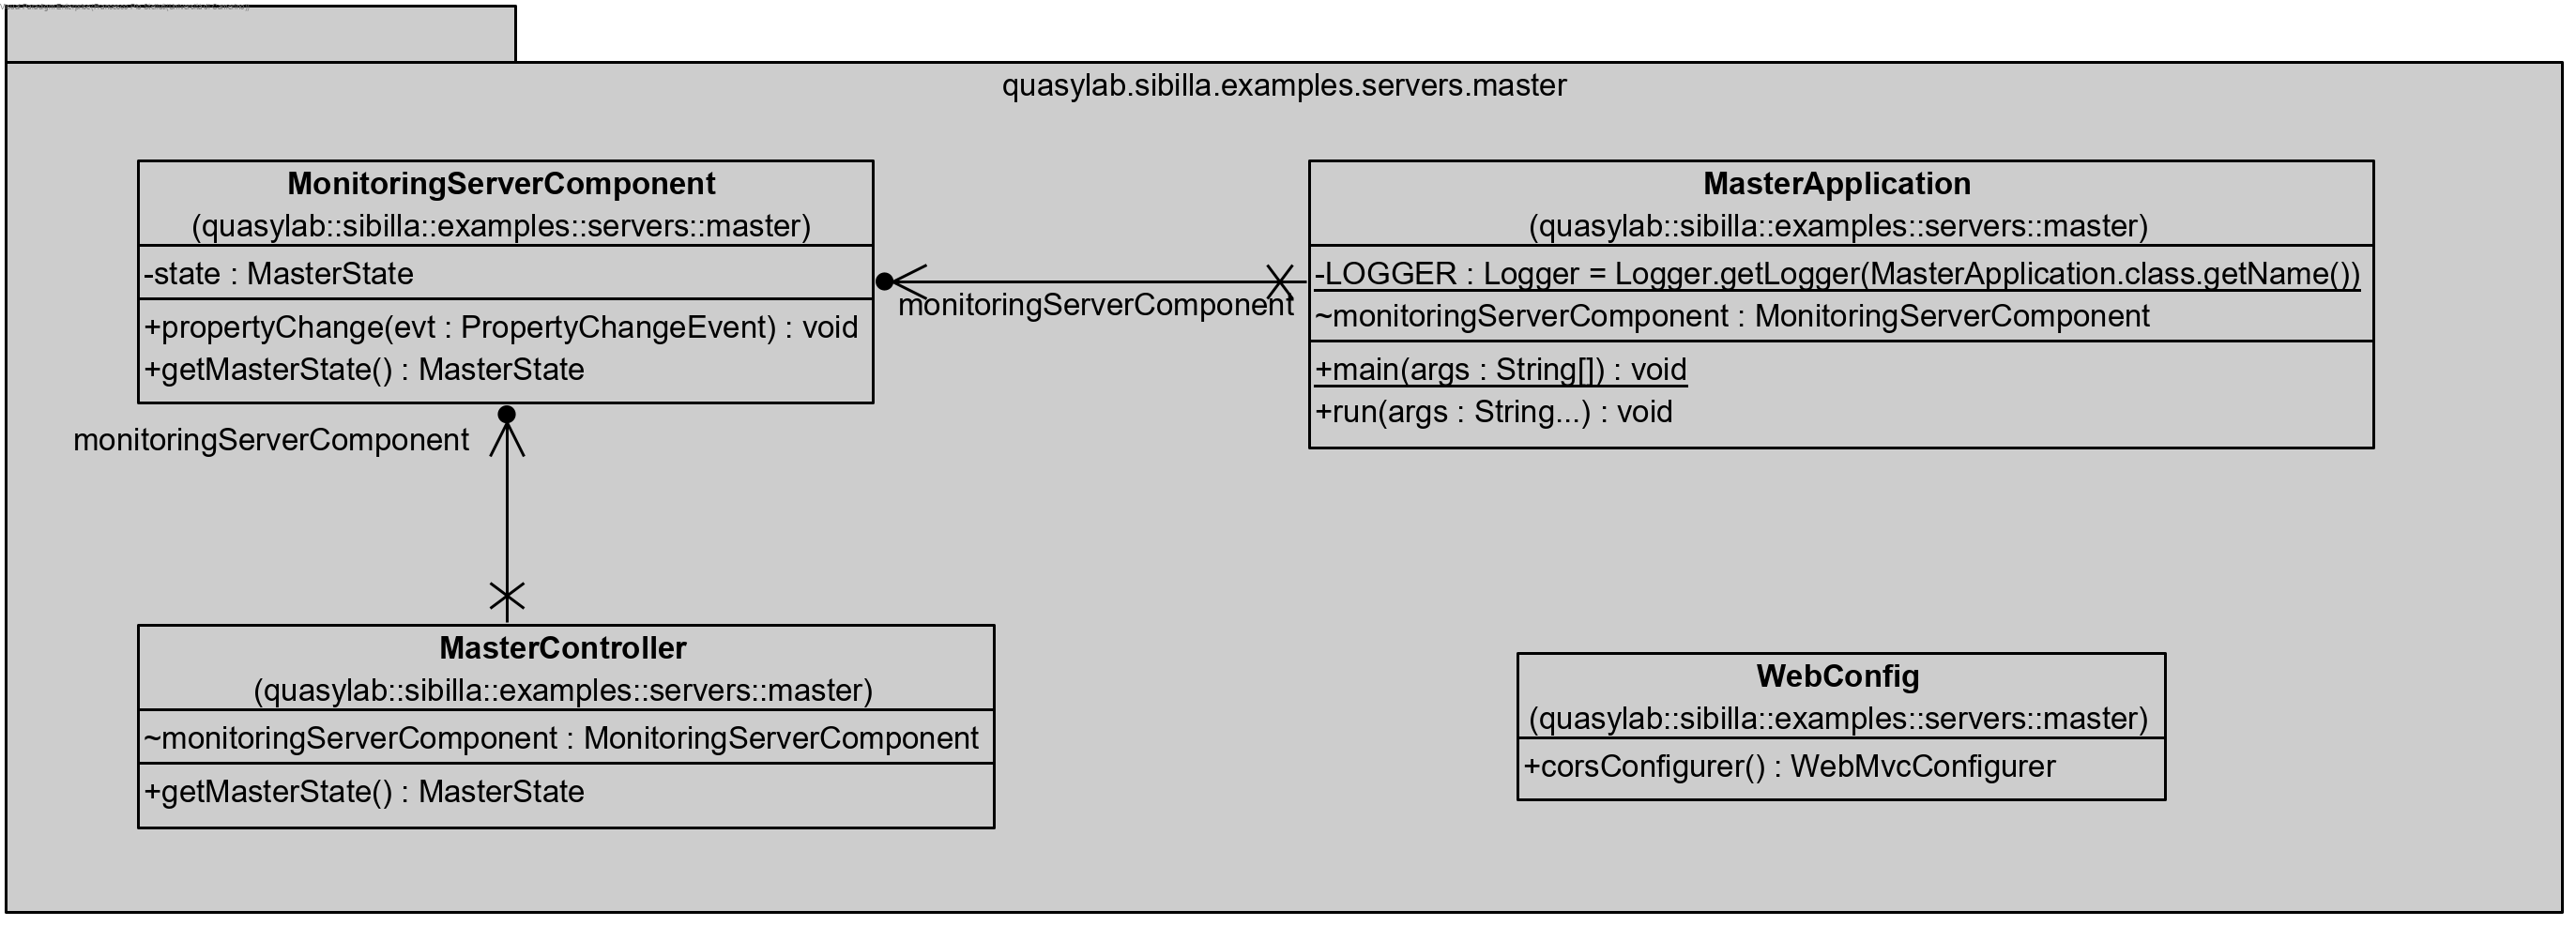
\includegraphics[width=\linewidth]{images/quasylab.sibilla.examples.servers.master.png}
    \captionsetup{justification=centering}
    \caption{Diagramma delle classi del package \texttt{quasylab.sibilla.examples.servers.master}}
  \end{figure}

\begin{table}[H]
    \begin{tabularx}{\linewidth}{ l X }
        \texttt{-keyStoreType}         & Il formato del keyStore per la connessione TLS              \\
        \texttt{-keyStorePath}         & Il path del keyStore per la connessione SSL                  \\
        \texttt{-keyStorePass}         & La password del keystore per la connessione TLS               \\
        \texttt{-trustStoreType}       & Il formato del trustStore per la connessione TLS            \\
        \texttt{-trustStorePath}       & Il path del trustStore per la connessione TLS                \\
        \texttt{-trustStorePass}       & La password del trustStore per la connessione TLS            \\
        \texttt{-masterDiscoveryPort}  & La porta locale utilizzata per il discovery dei server slave \\
        \texttt{-slaveDiscoveryPort}   & La porta remota utilizzata per il discovery dei server slave \\
        \texttt{-masterSimulationPort} & La porta locale utilizzata per gestire le simulazioni        \\
        \texttt{-slaveDiscoveryCommunicationType}   & Il tipo di comunicazione UDP utilizzata per il discovery dei server slave {[}DEFAULT{]}     \\
        \texttt{-clientSimulationCommunicationType} & Il tipo di comunicazione TCP utilizzata per gestire le simulazioni tramite i server slave {[}DEFAULT/SECURE{]}
    \end{tabularx}
    \captionof{table}{Parametri di avvio nel server master d'esempio}
\end{table}

\subsubsection{\texttt{quasylab.sibilla.examples.servers.slave}}

L'inizializzazione di un nuovo server slave è demandata alla classe \texttt{SlaveApplication}, all'interno della quale viene inizializzata un'istanza di \texttt{DiscoverableBasicSimulationServer} e vengono trattati i parametri di avvio specificati.
In aggiunta, nella cartella \textbf{resources} sono presenti i file \texttt{slaveKeyStore.jks} e \texttt{slaveTrustStore.jks}, relativi rispettivamente al keystore di chiavi private e al truststore delle chiavi pubbliche fidate associate allo server slave che si intende avviare. Tali file sono caricati dinamicamente da Gradle e consentono di impostare correttamente una connessione sicura tramite TLS, quando richiesta dall'utente all'avvio, senza ulteriori configurazioni.

\begin{figure}[H]
    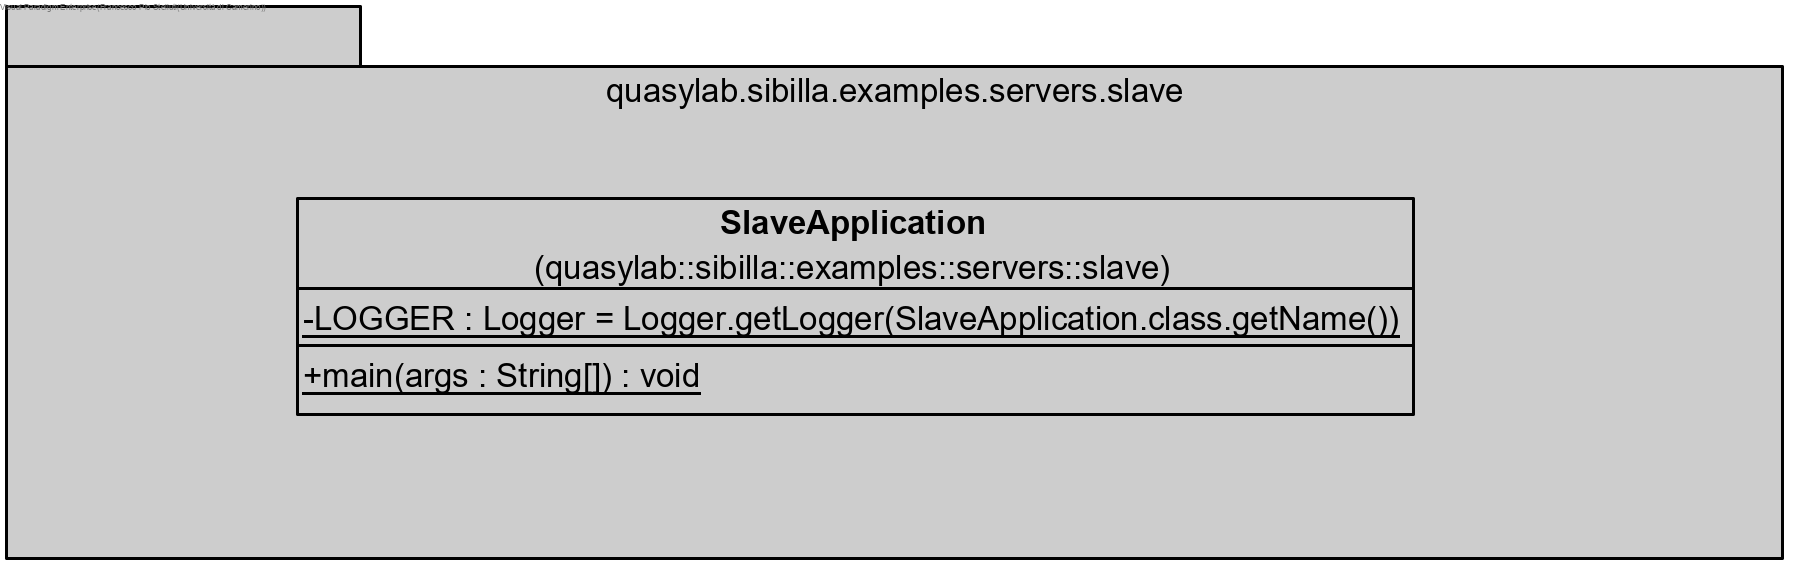
\includegraphics[width=\linewidth]{images/quasylab.sibilla.examples.servers.slave.png}
    \captionsetup{justification=centering}
    \caption{Diagramma delle classi del package \texttt{quasylab.sibilla.examples.servers.slave}}
  \end{figure}

\begin{table}[H]
    \begin{tabularx}{\linewidth}{ l X }
        \texttt{-keyStoreType}        & Il formato del keyStore per la connessione TLS       \\
        \texttt{-keyStorePath}        & Il path del keyStore per la connessione TLS           \\
        \texttt{-keyStorePass}        & La password del keystore per la connessione TLS        \\
        \texttt{-trustStoreType}      & Il formato del trustStore per la connessione TLS     \\
        \texttt{-trustStorePath}      & Il path del trustStore per la connessione TLS         \\
        \texttt{-trustStorePass}      & La password del trustStore per la connessione TLS     \\
        \texttt{-slaveDiscoveryPort}                & La porta locale utilizzata per il discovery da parte del server master                                              \\
        \texttt{-slaveSimulationPort} & La porta locale utilizzata per gestire le simulazioni \\
        \texttt{-masterDiscoveryCommunicationType}  & Il tipo di comunicazione UDP utilizzata per il discovery da parte dei server master {[}DEFAULT{]}               \\
        \texttt{-masterSimulationCommunicationType} & Il tipo di comunicazione TCP utilizzata per gestire le simulazioni col server master {[}DEFAULT/SECURE{]}
    \end{tabularx}
    \captionof{table}{Parametri di avvio nel server slave d'esempio}
\end{table}